\chapter{Selective sequencing}

\label{kap:selSeq} % id kapitoly pre prikaz ref

In this chapter, we are going to describe what is selective sequencing. We
show advantages that this method brings, the main challenges and current state of
research in this area.

\section{DNA sequencing}

% TODO: pridat zdroj %https://en.wikipedia.org/wiki/Genetics#DNA_sequencing_and_genomics
Genetics is a branch of biology that studies genes, genetic variation, and heredity.
It tries to explain the variability between animals, the source of hereditary diseases, and
other important things that influence our lives. DNA is the key molecule
that stores biological information. It is contained almost in every living cell. Based
on the information from this molecule our cells can reproduce and create copies of
themselves. Nowadays, it is possible to look at the DNA of the organism. This is
one of the strongest tools of genetics as it helps us tell what are the functions
of different parts of DNA by comparing it between organisms and looking at the
consequences of different mutations. DNA stores genetic information using a sequence of
nucleotides. Their particular order defies the stored information. There are four types of DNA nucleotides:
adenine(A), cytosine(C), guanine(G) and thymine(T). In fact, DNA consists of two long
molecules of these nucleotides. However, these two molecules are connected together
in a complementary way. So if on one string there is an A, then on the other
one must be T. If there is a C then on the other string we can expect
it's complement G. For the organisms it means that they can (to some extent) repair
missing nucleotides based on the complement rules. From now, we will for simplicity
assume that DNA sequence is a string of A, C, G, T. This representation is quite accurate
and we can also recover the other complementary DNA string easily. The process of obtaining DNA
sequence is called DNA sequencing. Example how we can think of DNA is on \ref{obr:acgt}.

% TODO: obrazok zdroj https://www.genome.gov/genetics-glossary/acgt

\begin{figure}
\centerline{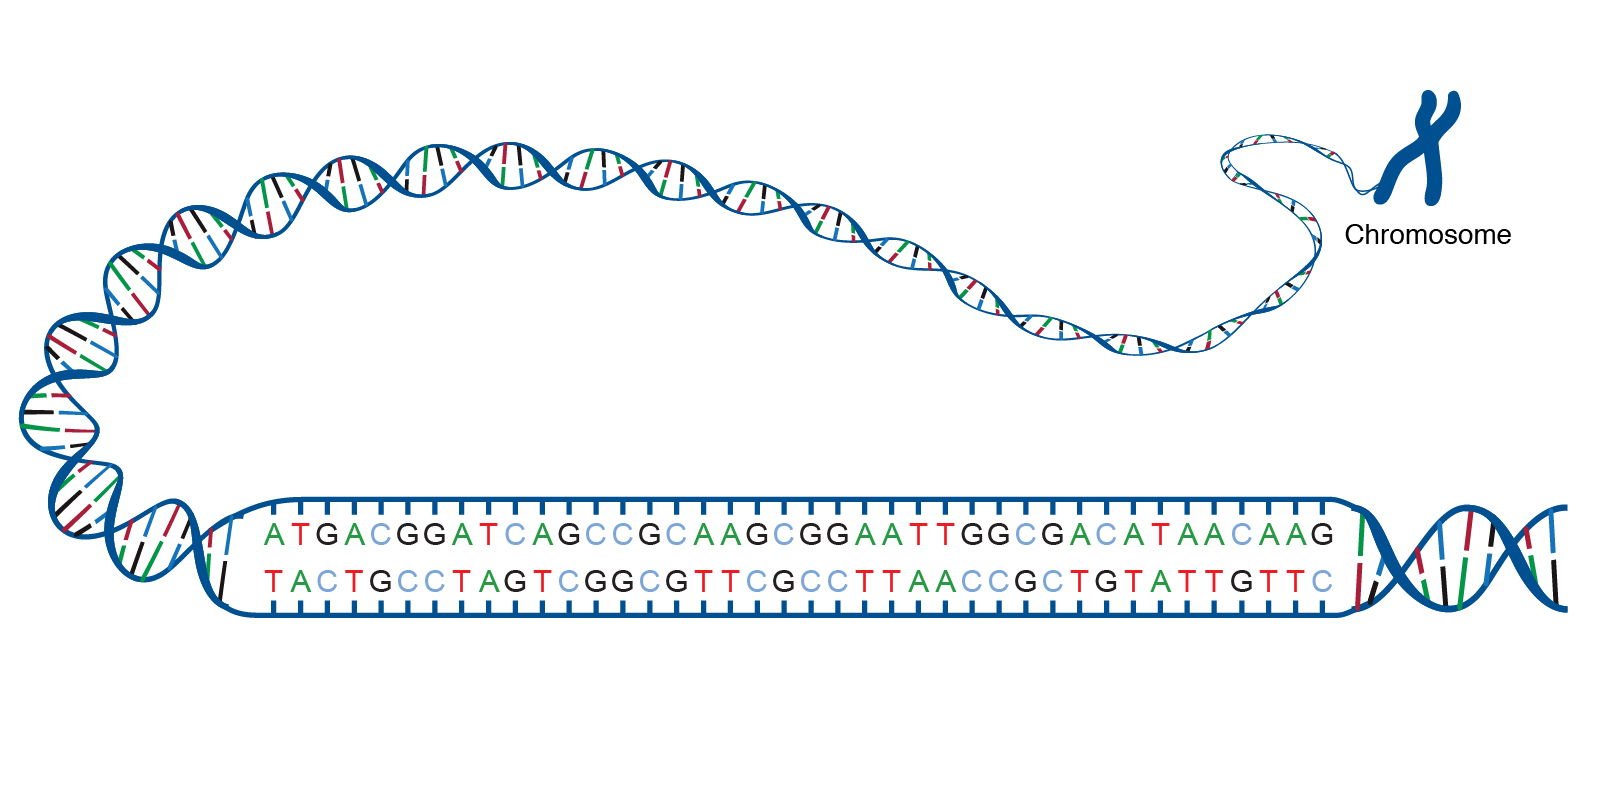
\includegraphics[width=0.7\textwidth, height=0.3\textheight]{images/acgt}}
\caption[DNA]{DNA Molecule}
\label{obr:acgt}
\end{figure}

The DNA molecule is very long and processing it whole would be very hard. Single
DNA molecule in one cell can reach up to 2 meters when untangled.
%https://www.sciencefocus.com/the-human-body/how-long-is-your-dna/
Thus, it is convenient to broke down the whole DNA molecule into many shorter parts.
This can be done chemically but it brings some problems, especially some of the
DNA molecules could be missed during sequencing so we would lose information about
that part of DNA. Because of this, we use DNA polymerases to duplicate these shorter DNA sequences
many times so we end up with a mixture containing our DNA molecule, broken into
many duplicated parts. DNA polymerases can stick to DNA molecule and rebuild the complementary
part. Once we have this mixture of shorter DNA molecules we need to sequence individual
parts and then somehow connect them together to obtain the nucleotide string representing
our DNA molecule.

One of the devices that serve this purpose is MinION\cite{lu2016oxford}. MinION is
a cheap and versatile DNA sequencer with the size of the modern smartphone showed in fig.
\ref{obr:minIon}.

\begin{figure}
\centerline{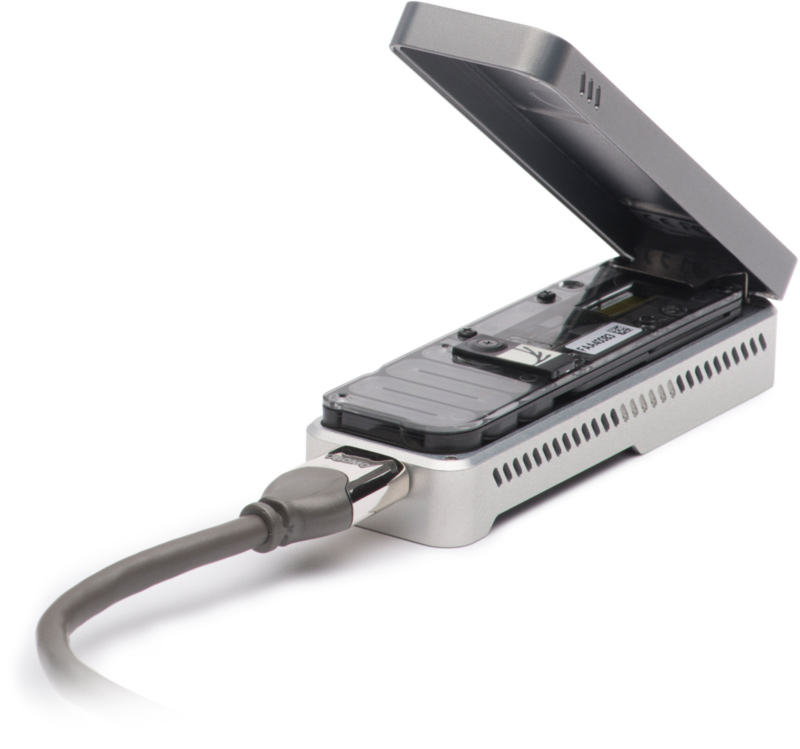
\includegraphics[width=0.7\textwidth, height=0.3\textheight]{images/minion}}
\caption[MinION]{MinION sequencer}
\label{obr:minIon}
\end{figure}

This sequencer consists of an active surface filled with pores. A pore is a small
hole with an electric current passing through it. The DNA molecule, negatively charged
will start to pass through the pores when the positive charge is generated on the
other side of the surface. As the molecule of DNA is passing through the pore of
MinION, we can observe changes in the flow of an electric current passing through the pore.
This electric current called signal is measured over the discrete-time. The example
of this signal is on figure \ref{obr:minIonCurrent}.

\begin{figure}
\centerline{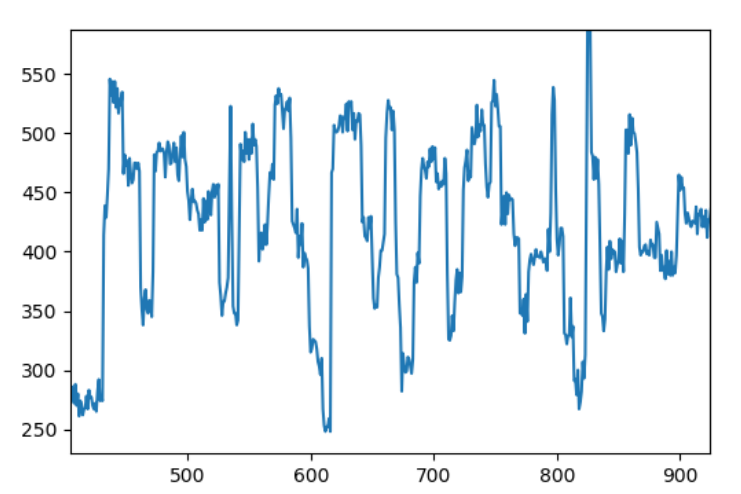
\includegraphics[width=0.7\textwidth, height=0.3\textheight]{images/signal}}
\caption[MinION signal]{Electric current (signal) coming from MinION.}
%id obrazku, pomocou ktoreho sa budeme na obrazok odvolavat
\label{obr:minIonCurrent}
\end{figure}

The minION version we use for the DNA sequencing process around 400 nucleotides per second.
The value of the signal is measured around 4000 times per second so it is good to
estimate that one nucleotide is on average measured about 10 times. Additionally,
minION has several these active pores and it can process several DNA molecules in
parallel. The signal generated from the pass of the single DNA molecule through
the single pore is called read.

When we obtain the signal from the pore, we need to convert it into the DNA
sequence. What is crucial for transcription of the signal into the DNA sequence is
that as the molecule of DNA is passing through the pore, only a small
number of nucleotides in the proximity of pore influence the output signal. So from
the measurements of signal throughout the time, using a method called base-calling,
we can tell how the molecule of DNA looked like. Despite big improvements in the
base-calling algorithms, the overall process of base-calling is quite slow and
resource-intensive.

\section{Selective sequencing}

MinION has a special ability that helps us in certain scenarios. It can reject
DNA molecule that is currently passing through the pore. MinION reverses the molecule’s direction and throws it away.
Selective sequencing is the idea that based on the incoming signal, we can tell
if we are interested in sequencing the current DNA molecule. Subsequently, we can decide if we want
to continue or reject this molecule. This happens on-the-fly so we need to make
the decision until the end of the current read. This often means we don't have time to
turn our signal into a nucleotide sequence as the reads are too short. This is
a reason why we have to work with a raw signal.

There are a lot of benefits of selective sequencing. In case we are not interested
in some DNA that we know is contained in our sample, we can use this technique to
reject unwanted DNA molecules. This saves us a lot of time and resources as obtaining
nucleotide sequence from the signal is in some scenarios unnecessary and too
costly process in terms of performance. With good selective sequencing, we only have
to further process reads we are interested in.

Let's say we are trying to find an exact type of virus in human blood. We can
reject all human DNA molecules because we are not interested in processing human
DNA. We could also filter positively. So we could say, that we are only
interested in sequencing DNA that produces a signal in some sense similar to our
chosen sample. This all means saving a lot of time and computing power in certain
cases, for example during the disease diagnosis process.

Naturally, there are some drawbacks to selective sequencing. In order to find out
if the currently passing molecule is from human DNA, we have to have some information
about the signal from human DNA beforehand.
This is of course in some sense limiting factor as we need a sample signal from
the species that we want to filter. The other problem is that in the case of misclassifying
some signal as not interesting, we lost information about the corresponding
part of the DNA molecule.

The idea of doing selective sequencing during the phase of reading the DNA molecules
(not as a part of some post-processing) is called Read Until. 

\section{Current state of selective sequencing}

%https://www.nature.com/articles/nmeth.3930
%https://www.biorxiv.org/content/10.1101/038760v1

There was some work regarding selective sequencing, most notably \cite{loose2016real}. In their
work, they obtain the reference signal using simulation from reference nucleotide
string. They use dynamic time warping (DTW) to align the signal from the read to
this reference signal. The DTW is a dynamic programming algorithm that takes two signals and aligns them in a
way that minimizes the total number of insertions and deletions. One of the limitations
of DTW is that it has run time complexity $\mathcal{O}(n\cdot m)$ where $n$ and $m$
is the length of the reference signal and read respectively. This poses a problem
for this method if we wanted to use it for a longer sequences...
